\documentclass[12pt,a4paper, xcolor=table]{article}
\usepackage{graphicx}
\usepackage[utf8]{inputenc}
\usepackage{eurosym}
\usepackage[spanish,es-tabla]{babel}
\usepackage[left=2cm, right=2cm, top=2cm, bottom=2cm]{geometry}
\usepackage{afterpage}
\PassOptionsToPackage{hyphens}{url}\usepackage{hyperref}
\usepackage{subfig}
\usepackage[table,xcdraw]{xcolor}
\usepackage{cite}
\usepackage{url}
\usepackage{changepage}

\usepackage{imakeidx}
\newcommand\blankpage{%
    \null
    \thispagestyle{empty}%
    \addtocounter{page}{-1}%
    \newpage}
\renewcommand*\contentsname{Índice: }

\makeindex
\let\olditemize\itemize
\def\itemize{\olditemize\itemsep=0pt}

\begin{document}
\setlength{\parindent}{0pt}
\begin{titlepage}
        \centering
        
\includegraphics[width=0.75\textwidth]{img/logo_uc3m.jpg}\par\vspace{2cm}
        {\huge\bfseries Práctica Final \\ Predicción del género de libros\par}
        \vspace{0.5cm}
        {\scshape\Large Inteligencia Artificial en las Organizaciones\par}
        \vspace{1.5cm}
        {\scshape\Large Grupo 83-1\par}
        \vspace{1.5cm}
        {\Large\itshape Miguel Gutiérrez Pérez\par}
        {\Large 100383537@alumnos.uc3m.es \par}
        \vspace{1cm}
        {\Large\itshape Mario Lozano Cortés\par}
        {\Large 100383511@alumnos.uc3m.es\par}
        \vspace{1cm}
        {\Large\itshape Alba Reinders Sánchez\par}
        {\Large 100383444@alumnos.uc3m.es\par}
        \vspace{1cm}
        {\Large\itshape Alejandro Valverde Mahou\par}
        {\Large 100383383@alumnos.uc3m.es\par}
        \vspace{5mm}
        {\large GitHub: \textbf{\textit{\href{https://github.com/Pheithar/InteligenciaArtificialOrganizaciones}{InteligenciaArtificialOrganizaciones}}}}
        \vfill

% Bottom of the page
        {\large \today\par}
\end{titlepage}

\tableofcontents

\newpage

\section{Introducción}

El objetivo de esta práctica consiste en abordar una clasificación sobre resúmenes de libros para determinar su género literario. Las razones que llevan a la elección de este problema tienen que ver con que actualmente cualquier persona con la dedicación suficiente puede escribir un libro sin la necesidad del patrocinio de una editorial, lo que conlleva una \textbf{explosión en el número de nuevos libros generados}. Por consiguiente, las librerías y bibliotecas necesitan catalogar una gran cantidad de escritos, lo cual, les lleva a necesitar de métodos de clasificación automática. Por ello, se plantea el uso de resúmenes y metadatos de los libros puesto que la tarea de clasificación \textbf{debe poder realizarse con el menor número de datos posible}, puesto que no todos los libros que llegan a estas entidades disponen de todos los datos completos.

\vspace{3mm}

La primera cuestión imprescindible que surge al conocer el problema propuesto es qué técnica de Inteligencia Artificial emplear. Dado que se realiza un análisis sobre diferentes textos, la opción evidente es la \textbf{Minería de Texto}, la cual es una técnica de minería de datos que busca extraer \textbf{información útil y relevante de documentos de texto} de diferentes fuentes diferentes, como puede ser páginas web,
correos electrónicos, periódicos o redes sociales. Para ello, se hace una identificación de patrones en los datos, como puede ser la repetición de palabras o conjuntos de palabras, estructuras sintácticas que se repitan a lo largo de los datos, etc. Esta minería de texto tiene numerosas aplicaciones, y en esta práctica se van a desarrollar una clasificación en función de unas categorías que serán definidas gracias a la elección de un dataset apropiado.

\vspace{3mm}

A continuación se ofrece un\textbf{ esquema del funcionamiento de la tarea propuesta }en donde un libro sin catalogación llega a alguna a de estas entidades que necesitan catalogar su género a partir de la información más reducida posible (generalmente título y argumento). Inicialmente se plantea la distinción de un único género, sin embargo, \textbf{es bien sabido que un escrito no tiene por qué adscribirse a un único género} y por lo tanto se debe considerar como futura \textbf{ampliación} catalogar tantos como sea posible.

\vspace{12mm}

  \begin{figure}[!h]
    \centering
    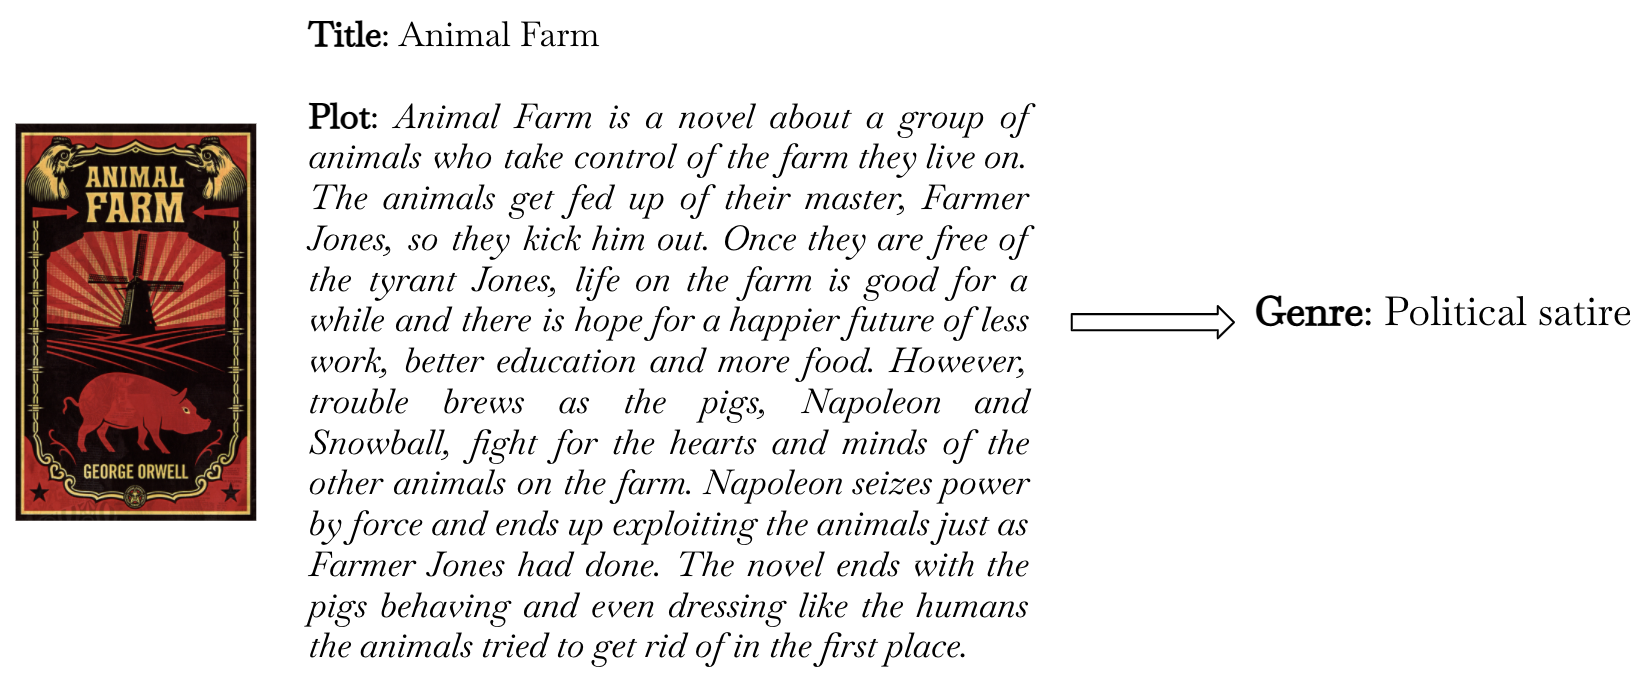
\includegraphics[width=450px]{img/Animal Farm.png}
    \caption{Esquema de la tarea}
    \end{figure}

\newpage

\section{Conceptos teóricos}
A la hora de elegir un método de Minería de Textos se consideran diversas opciones tales como utilizar la herramienta Weka de la Universidad de Waitako, sin embargo, dado que esta herramienta ya ha sido utilizada a lo largo de la asignatura a la que se adscribe este trabajo y además presenta ciertas limitaciones en cuanto a la flexibilidad y capacidad de toma de decisiones de diseño en los modelos se decide aplicar Word Embedding en redes de neuronas con la biblioteca de código abierto Tensorflow. De esta manera se usará un método diferente al usado en clase, lo cual permite experimentar y aprender tecnologías nuevas. 

\vspace{3mm}

No obstante, antes de iniciar la codificación de algún modelo, dado que se trata de una técnica nueva es necesario tener claros los conceptos teóricos involucrados. Una red neuronal únicamente procesa números, lo que implica que es necesario realizar una transformación. Representar las palabras como vectores es importante, ya que los modelos de inteligencia artificial no ‘entienden’ las palabras, y no puede realizar cálculos ni aprendizaje sobre ellas. Por este motivo, es necesario realizar una vectorización, que no es más que transformar estas palabras en números, agrupados en forma de vector. A continuación se exponen las diferentes técnicas de vectorización consideradas.

\subsection{Codificación con valor único}
Una primera aproximación podría ser asignar un único número a cada una de las palabras consideradas en la vectorización. Así si por ejemplo, se tiene la frase "hace un espléndido día" se obtiene un vector como el que sigue:

      \begin{table}[h]
        \centering
        \begin{tabular}{|c|c|}
        \hline
        \rowcolor[HTML]{DAE8FC}
        \textbf{Palabra} & \textbf{Valor} \\ \hline
        hace                    & 1   \\ \hline
        un                     & 2   \\ \hline
        espléndido                     & 3  \\ \hline
        día                       & 4   \\ \hline
        \end{tabular}
        \caption{Codificación con un único valor}
            \label{fig:graf_exp1}
    \end{table}
    
Este enfoque presenta una serie de consideraciones importantes:
\begin{itemize}
\item El valor de cada palabra se decide de manera arbitraria.
\item No se obtiene una representación fiel de la distancia entre palabras, lo cual es un hecho que es importante en el desarrollo de esta práctica.
\end{itemize}

Por ello, se descarta el enfoque aquí propuesto por no ser eficiente en la tarea propuesta.

\subsection{One-hot encoding}
Al codificación one-hot consiste en convertir cada palabra en un vector con tantas posiciones como palabras tengamos, 1 en la posición que se corresponda a la palabra considerada y 0 en caso contrario. 

\vspace{2mm}

A continuación se muestra un ejemplo de la codificación con el pequeño set de palabras utilizado en la sección anterior.

  \begin{table}[h]
        \centering
        \begin{tabular}{|c|c|c|c|c|}
        \hline
        \textbf{} &\textbf{hace} & \textbf{un} & \textbf{espléndido} & \textbf{día}  \\ \hline
        \textbf{hace}                     & 1 & 0 & 0 & 0\\ \hline
        \textbf{un}                       & 0 & 1 & 0 & 0\\ \hline
        \textbf{espléndido}               & 0 & 0 & 1 & 0\\ \hline
        \textbf{día}                      & 0 & 0 & 0 & 1\\ \hline
        \end{tabular}
        \caption{One-hot encoding}
            \label{fig:graf_exp1}
    \end{table}

\vspace{2mm}

El principal problema de esta técnica de vectorización es que la distancia entre las palabras es la misma, lo cual impide de nuevo disponer de una representación realista de este hecho esencial en el enfoque que se propone.

\subsection{Embedding}

Está técnica sirve para representar aquellas \textbf{palabras que son semánticamente parecidas con una codificación similar}. Lo que hace esta técnica tan atractiva es que no es necesario especificar esta similitud de forma manual. Un \textit{embedding} es un vector denso de números reales, donde su longitud viene determinada por parámetro. En lugar de determinar los pesos a mano, se tratan como \textbf{parámetros que pueden ser entrenados}, como si de pesos de redes de neuronas densas se trataran. Por eso mismo, esta técnica funciona especialmente bien con las redes de neuronas, que incorpora la modificación de estos pesos a la fase de entrenamiento de la red.

\vspace{2mm}

La dimensionalidad del \textit{embedding} debe ser proporcional a la cantidad de datos disponibles, ya que cuanto más grande sea el vector, más detalles podrá obtener de cada palabra, pero requiere de más datos para ser entrenado. A continuación se muestra un ejemplo de la codificación con el pequeño set de palabras utilizado en la sección anterior.

  \begin{table}[h]
        \centering
        \begin{tabular}{|c|c|c|}
        \hline
        \textbf{hace}                     & 2.32 & 7.35 \\ \hline
        \textbf{un}                       & 0.89 & 4.23 \\ \hline
        \textbf{espléndido}               & 0.75 & 8.65 \\ \hline
        \textbf{día}                      & 2.65 & 3.00 \\ \hline
        \end{tabular}
        \caption{Embedding}
            \label{fig:graf_exp1}
    \end{table}

Por lo tanto esta técnica resulta de gran utilidad a la hora de conseguir representar la distancia semántica entre las palabras que forman un texto. Siendo este hecho fundamental para la tarea se propuesta \textbf{se decide apostar por esta codificación para construir el modelo de text mining}.
\section{Conclusiones}

\clearpage

\bibliographystyle{ieeetr}
\bibliography{bibliografia.bib}


\end{document}
